\documentclass[a4paper,13pt,oneside]{article}
 \usepackage[latin1]{inputenc}
 \usepackage[T1]{fontenc}
 \usepackage[english]{babel}
\usepackage{amssymb}
\usepackage{graphicx}
\usepackage{subfigure}
\usepackage{amsmath}
\usepackage{amsthm}
\usepackage{float}
\usepackage{tikz}
\usepackage{ragged2e}
\newtheorem*{claim}{Claim}

\theoremstyle{remark}
\newtheorem*{remark}{Remark}
\renewcommand*\abstractname{\flushleft\textbf{Abstract}\hfill}

\title{Betting on Catalan numbers}
\author{Dylan Da Silva Moreira, Hukic Ibrahim}
\begin{document}
\maketitle
\newpage
\abstract 

\section{Introduction }

		A fair coin is flipped $100$ times yielding a sequence $a = (a_1,\dots, a_{100})$ of Heads or Tails. Player A realizes that if one thinks of Heads as $+1$ and Tails as $-1$, then for each k\ in [1, 100], $\sum_{i=1}^{k} a_i \geq 0$.
		\\Furthermore, $\sum_{i=0}^{100} a_1=0$.
		\\Player B thinks such a sequence is extremely unlikely and offers a bet to A with a $100 : 1$ odds that if they flip the coin again $100$ times yielding a random sequence $x = (x_1,\dots, x_{100})$, then $x$ is not going to satisfy the properties of $a$. Should A accept the bet? What are the true odds for such an event? Is there a good graphical representation for the properties of $a$? What if there are $2n$ coin flips? Biased coin?
	
\pagebreak
\section{Experiment (Programming)}
\pagebreak
\section{Theoretical approach}


Let us redefine our $+1$,$-1$ random sequence into \textit{rightward} ($-1$) and \textit{upward} ($+1$) steps. The solution to our coin flip problem are all the paths that end on the straight line $f(x) = x$ (sum equals to zero) and don't cross the line at any given moment (sum being always positive).

\bigskip


\begin{center}

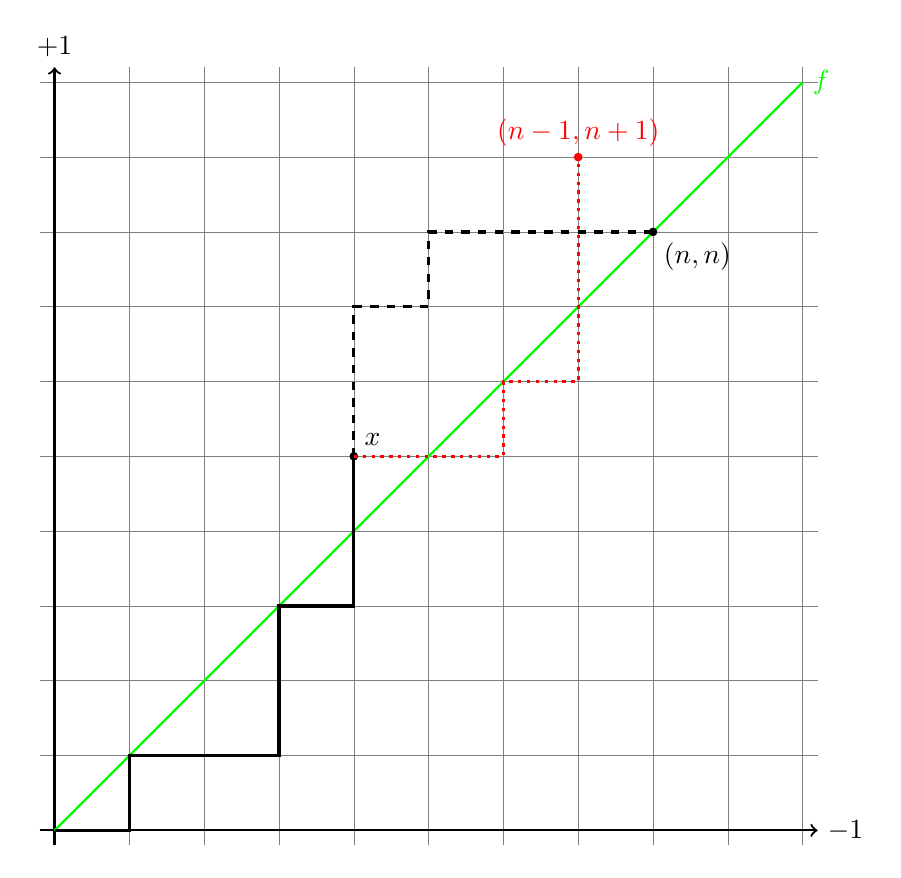
\begin{tikzpicture}[scale= 0.95]
\draw[gray, very thin] (-0.2,-0.2) grid (10.2,10.2);
\draw[->,thick] (-0.2,0) -- (10.2,0) node[right]{$-1$} ; 
\draw[->,thick] (0,-0.2) -- (0,10.2) node[above] {$+1$} ;
\draw[green ,thick] (0,0) -- (10,10) node[right] {$f$};
\draw [very thick](0,0) -- (1,0) -- (1,1) -- (3,1) -- (3,3) -- (4,3) --(4,5) node[above right] {$x$};
\draw [fill] (4,5) circle[radius=0.05];
\draw [dashed, very thick] (4,5) -- (4,7)--(5,7)--(5,8)--(8,8) node[below right]{$(n,n)$};
\draw [fill] (8,8) circle[radius=0.05];
\draw[dotted,very thick,red]   (4,5)--(6,5)--(6,6)--(7,6)--(7,9) node[above] {$(n-1,n+1)$};
\draw[fill,red] (7,9) circle[radius=0.05];
\end{tikzpicture}

\end{center}


\begin{claim} \label{claim}
The number of paths satisfying the above conditions is given by:
\[
\boxed{\binom{2n}{n} - \binom{2n}{n+1}  \quad ,n\in \mathbb{N}}
\]	
\end{claim}
\bigskip
\begin{remark}
A point on the line $f$ is denoted by $(n,n)$ where $n =\frac{l}{2}$ with $l$ being the length of the sequence.
\end{remark}
\bigskip
\begin{proof}
To end up at the point $(n,n)$ one has to choose $n$ \textit{upward} (or equivalently \textit{rightward}) steps out of $2n$ total steps. So the number of paths satisfying this condition is equal to : 
\[\binom{2n}{n}\] 
Considering this number still contains paths which will end on the line but cross it at a given moment we need to exclude them.
To find out the number of "bad paths" we will flip the portion of a path \underline{after}  it has crossed the line for the first time. By "flipping" one means interchanging all  \textit{upwards} and \textit{rightward} steps.
The section of a bad path which hasn't been flipped contains one more \textit{upwards} step than \textit{rightward} steps, hence the remaining path contains one more \textit{rightward} step than \textit{upward} step because it end on the line $f$. Since there are $2n$ steps and the flipping process doesn't change the total amount of steps , every flipped bad path will end at the point $(n-1,n+1)$.
Thus the number of bad paths is given by the possible permutations of $n+1$ \textit{upward} steps (or equivalently, $n-1$ \text{rightward} steps)  for a total of $2n$ steps : 
\[
\binom{n+1+n-1}{n+1} =\binom{2n}{n+1}= \binom{2n}{n-1}
\]

By subtracting  one finally obtains :
\[
\binom{2n}{n} - \binom{2n}{n+1}
\]


\end{proof}
\bigskip

Let us develop this expression furthermore :
\begin{align*}
\binom{2n}{n} - \binom{2n}{n+1} &= \frac{(2n)!}{n! \, (2n-n)!} - \frac{(2n)!}{(n+1)! \, (2n-n-1)!}\\
&= \frac{(2n)!}{n! \, (2n-n)(2n-n-1)!} - \frac{(2n)!}{(n+1)\,n! \, (2n-n-1)!}\\
&= \frac{(2n)! \, (n+1-2n+n)}{n!\,(2n-n-1)!\,(2n-n)(n+1)}\\
&=\frac{(2n)!}{n!\,(2n-n-1)!\,(2n-n)(n+1)}\\
&= \frac{(2n)!}{n!\,(2n-n)!\,(n+1)} = \frac{(2n)!}{(n+1)! \,n!}\\
&= \frac{1}{1+n} \binom{2n}{n}
\end{align*}

\begin{flushleft}
One realizes that this is the formula for the \textbf{Catalan numbers}, which is a sequence of natural numbers given by :
\[ 
\boxed{C_n = \frac{1}{1+n} \binom{2n}{n}= \frac{(2n)!}{(n+1)! \,n!}=\prod_{k=2}^{n} \frac{n+k}{k} \qquad \text{for} \:n \geq 0.}
\]
\end{flushleft}
\pagebreak


\end{document}
